\section{Power Dissipation in Resistors}

\instructornote{%
By Matt Trawick, 2015.  Time: maybe an hour?

This is admitedly not the most sophisticated investigation we do, but several students have said this was their favorite lab all semester.

This lab assumes that students have already seen $P=IV$.  But for most students, just being introduced to it doesn't really teach them what power MEANS, in the very visceral sense of things becoming hot to the touch.

Equipment notes: 

I believe the circuits here are most easily (and intuitively) constructed using banana cables, with aligator clips used for the connections to the resistors themselves.  For the resistors, use 100 ohm resistors.  I've typically used:
 1/8 watt
 1/4 watt (sometimes)
 2 or 3 watt,
and  25 watt

The very smallest resistors can actually catch on fire, with a small burst of flame about a tenth as big as a match, say, so be prepared.  The 2 watt resistors will smoke and turn brown.  The biggest power resistors are totally unharmed.  By the way, it's always more memorable for the students if you don't tell them about the catching on fire part until it actually happens.

I try to have at least one of the ones in the middle have a positive temperature coefficient (metal film) and one have a negative temperature coefficient (carbon glass).

For the multimeters, have plenty of extra fuses on hand, as some fuses will be blown!
}

\makelabheader %(Space for student name, etc., defined in master.tex)

\textbf{Apparatus}
\begin{itemize}
\item digital multimeters (2)
\item DC power supply 
\item various resistors
\item banana cables and aligator clips
\end{itemize}

\textbf{Activity 1: Measuring Resistances}

(a) You have at your lab station a bunch of different resistors.  Use the color table below to help you read the ``nominal'' value of each resistor.  Then measure the actual resistance of each resistor using your digital multimeter (DMM).  (Set the DMM to ``$\Omega$'' and put the two leads in the jacks labeled ``COM'' and ``V-$\Omega$''.)

\begin{center}
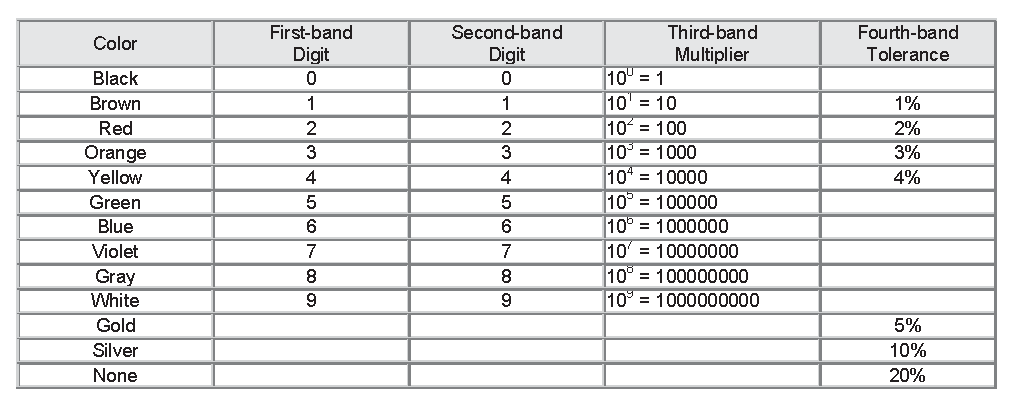
\includegraphics[width=1.0\textwidth]{electric_power/color_code.eps}

\vspace{0.2in}
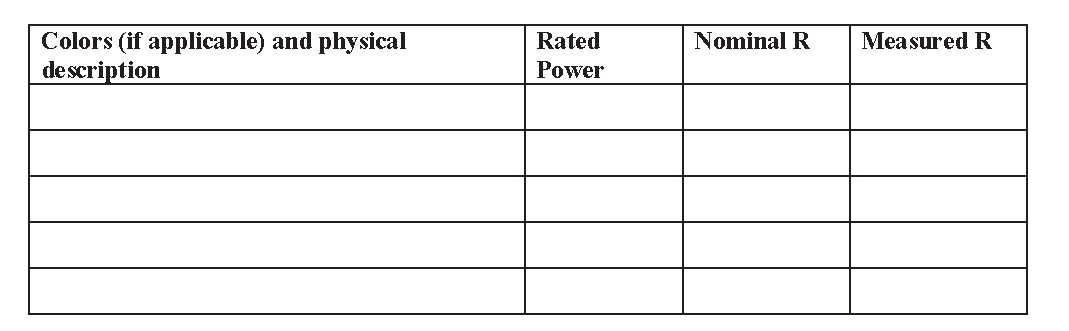
\includegraphics[width=1.0\textwidth]{electric_power/resistor_description.eps}
\end{center}

(b) What is the relationship between the physical size of the resistors and their resistance?
\vspace{1.0in}

\pagebreak
\textbf{Activity 2: Measuring Voltage, Current, and Power}

\begin{wrapfigure}[8]{r}{0.3\textwidth}
    \vspace{-0.4 in}
    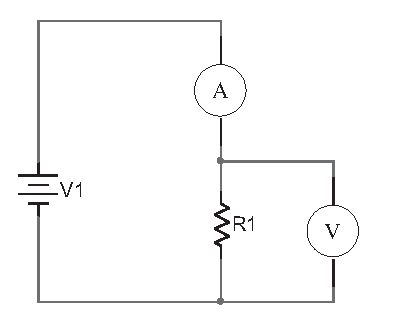
\includegraphics[width=0.3\textwidth]{electric_power/circ_diagram_bw.eps}
\end{wrapfigure}

(a) Connect the physically largest resistor to the power supply as shown in the circuit diagram to the right, using two multimeters to precisely measure both the current $I$ and the voltage drop $\Delta V$ across the resistor.  As you increase the voltage across the resistor, calculate both the power $P$ dissipated in it, and its resistance as calculated by $\Delta V/I$.  At each value, feel the resistor (\textit{carefully, so you don't burn your fingers!}) to see if it is getting hot.  To get accurate current readings, use the smallest current range you can, but do not exceed the maximum current of that range, or you may blow a fuse.

\begin{center}
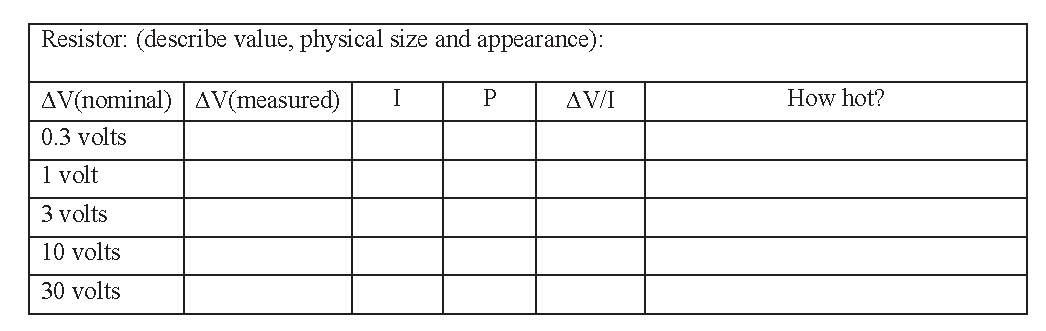
\includegraphics[width=1.0\textwidth]{electric_power/iv_table.eps}
\end{center}

(b)  Based on your measurements, did the resistance increase, decrease, or stay the same as you increased the current?  (Be careful: are your measurements of current and voltage precise enough to support your conclusion?)  Is the temperature coefficient positive or negative for this resistor? 
\vspace{1.5in}

\begin{center}
\framebox[1.07\width]{\textit{This is a good time to check with your instructor to be sure your measurements are on the right track.}} \par
\end{center}

(c) Now repeat your measurements for each of the other resistors, recording results in the tables below.  \textit{Again, be careful not to burn your fingers!}
\begin{center}
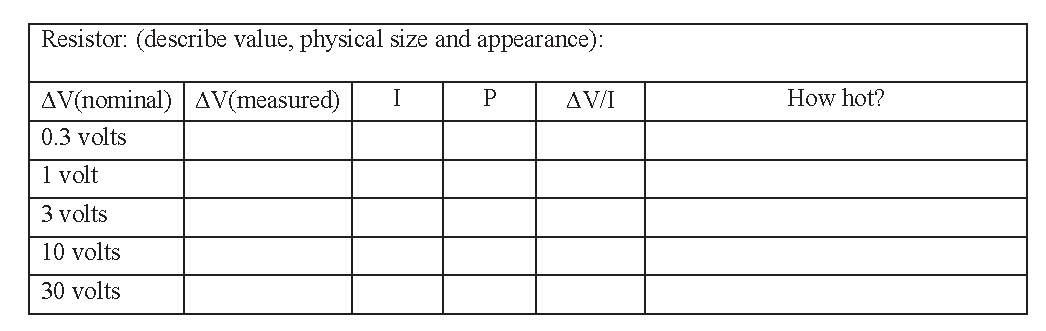
\includegraphics[width=1.0\textwidth]{electric_power/iv_table.eps}
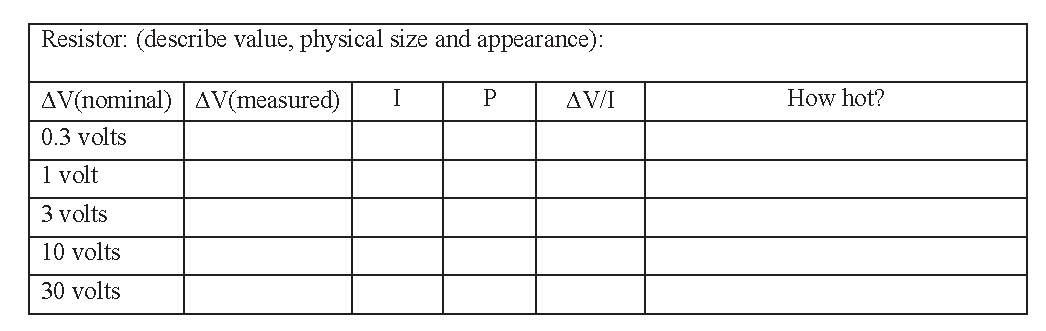
\includegraphics[width=1.0\textwidth]{electric_power/iv_table.eps}

\vspace{0.5in}
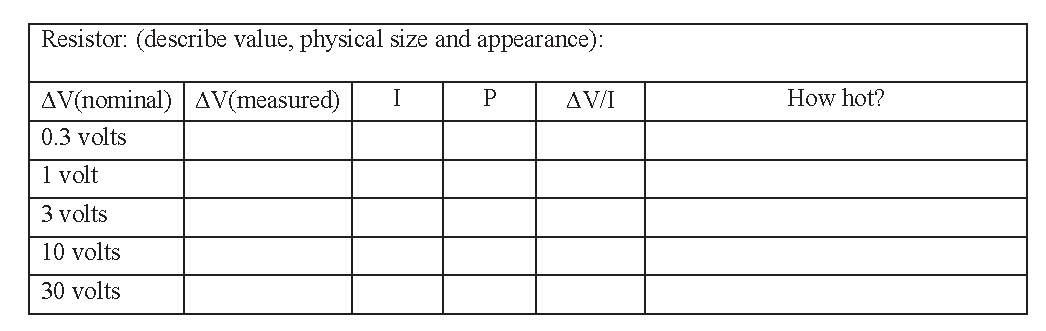
\includegraphics[width=1.0\textwidth]{electric_power/iv_table.eps}
\end{center}

(d) Now that they are no longer hot, make a final resistance measurement of each resistor (or whatever is left of it).  Have any of their resistances changed permanently?
\vspace{1.5in}

(e) What difference does physical size of the resistor make in the results of any of your measurements?  Why?
\vspace{1.5in}






